\newpage
\subsection{QuizziPedia::Front-End::Services}
\begin{figure}
	\centering
	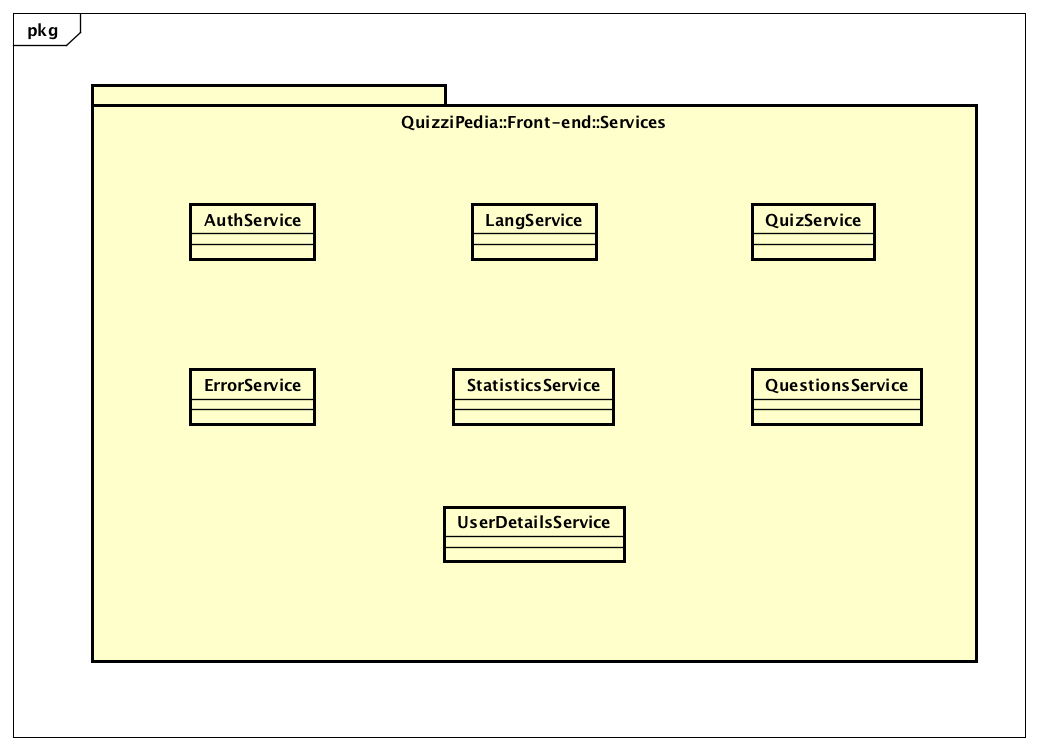
\includegraphics[scale=0.45]{UML/Package/QuizziPedia_Front-End_Services.png}
	\caption{QuizziPedia::Front-End::Services}
\end{figure}
\subsubsection{Informazioni generali}
\begin{itemize}
	\item \textbf{Descrizione}: package che contiene le classi individuate che permettono la comunicazione del lato front-end con il lato back-end;
	\item \textbf{Padre:} \texttt{Front-End};
	\item \textbf{Interazione con altri componenti:}
	\begin{itemize}
		\item \texttt{Models} - package che contiene le classi model individuate;
		\item \texttt{Controllers} - package che contiene le classi controller individuate.
	\end{itemize} 
\end{itemize}
\subsubsection{Classi}

\paragraph{QuizziPedia::Front-End::Services::AuthService}
\begin{figure}
	\centering
	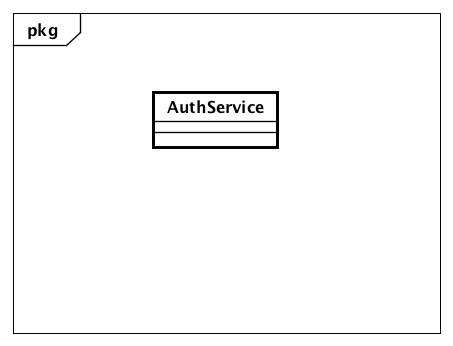
\includegraphics[scale=0.45]{UML/Classi/Front-End/QuizziPedia_Front-end_Services_ AuthService.png}
	\caption{QuizziPedia::Front-End::Services::AuthService}
\end{figure}
\begin{itemize}
	\item \textbf{Descrizione}: questa classe permette di gestire la registrazione e l'autenticazione di un utente;
	\item \textbf{Utilizzo}: fornisce le funzionalità di registrazione e autenticazione ai controllers. Controlla che i dati inseriti dall'utente siano presenti nel \textit{Database\ped{G}} in caso di autenticazione. Presenta anche le funzionalità per la gestione del reset della password;
	\item \textbf{Relazione con altre classi:}
	\begin{itemize}
		\item \textit{OUT} \texttt{LoginController}: questa classe gestisce la logica alla base della pagina di autenticazione;
		\item \textit{OUT} \texttt{LogoutController}: questa classe permette di gestire la pagina di logout;
		\item \textit{OUT} \texttt{PasswordForgotController}: questa classe gestisce la logica alla base del reset della password;
		\item \textit{OUT} \texttt{SignUpController}: questa classe gestisce la logica alla base della registrazione di un nuovo utente.
	\end{itemize}
	\item \textbf{Attributi:}
	\begin{itemize}
		\item \texttt{-} \texttt{logged: Boolean}: campo dati che indica se l'utente è autenticato;
		\item \texttt{-} \texttt{\$http: \$http}: campo dati che contiene un riferimento al servizio \$http che permette la comunicazione con il protocollo HTTP;
		\item \texttt{-} \texttt{\$q: \$q}: campo dati che contiene un riferimento a \$q, un servizio offerto da \textit{Angular\ped{G}} per la gestione, tramite \textit{Promise\ped{G}}, di chiamate asincrone.
	\end{itemize}
	\item \textbf{Metodi:}
	\begin{itemize}
		\item \texttt{+} \texttt{isLogged(): Boolean} \\ Metodo che restituisce ln valore dell'attributo \textit{logged};
		\item \texttt{+} \texttt{signin(username: String, password: String): Promise}\\ Metodo che permette di effettuare il login all'applicazione facendo una richiesta di autenticazione al back-end passando i parametri ricevuti. Il metodo ritorna una \textit{Promise\ped{G}}. In caso la \textit{Promise\ped{G}} venga rifiutata, verrà restituito al \texttt{LoginController} un oggetto \texttt{ErrorModelInfo} contenente tutti i dettagli dell'errore; \\
			\textbf{Parametri}: 
			\begin{itemize}
				\item \texttt{username: String}: parametro che rappresenta lo username o la email dell'utente;
				\item \texttt{password: String}: parametro che rappresenta la password dell'utente.
			\end{itemize}
		\item \texttt{+} \texttt{logout(username: String): Promise} \\ Metodo che permette di effettuare il logout dall'applicazione. Il metodo ritorna una \textit{Promise\ped{G}}. In caso la \textit{Promise\ped{G}} venga rifiutata, verrà restituito al \texttt{LogoutController} un oggetto \texttt{ErrorModelInfo} contenente tutti i dettagli dell'errore; \\
		\textbf{parametri}:
		\begin{itemize}
			\item \texttt{username: String}: parametro che rappresenta l'utente che vuole eseguire il logout.
		\end{itemize}
		\item \texttt{+} \texttt{signup(username: String, password: String, email: String, nome: String, cognome: String): Promise} \\Metodo che permette di effettuare la registrazione all'applicazione tramite richiesta di creazione nuovo account al back-end. Il metodo ritorna una \textit{Promise\ped{G}}. In caso la \textit{Promise\ped{G}} venga rifiutata, verrà restituito al \texttt{SignUpController} un oggetto \texttt{ErrorModelInfo} contenente tutti i dettagli dell'errore. \\
			\textbf{parametri}:
			\begin{itemize}
				\item \texttt{username: String}: parametro che rappresenta lo username o la email dell'utente;
				\item \texttt{password: String}: parametro che rappresenta la password dell'utente;
				\item \texttt{email: String}: parametro che rappresenta la email dell'utente;
				\item \texttt{nome: String}: parametro che rappresenta il nome dell'utente;
				\item \texttt{cognome: String}: parametro che rappresenta il cognome dell'utente.
			\end{itemize}
		\item \texttt{+} \texttt{getNewPassword(email: String): Void}  \\Metodo che permette il recupero della password. \\
			\textbf{Parametri}:
			\begin{itemize}
				\item \texttt{email: String}: parametro che rappresenta la mail a cui mandare una mail per resettare la password.
			\end{itemize}
	\end{itemize}
\end{itemize}


\paragraph{QuizziPedia::Front-End::Services::SearchService}
\begin{figure}
	\centering
	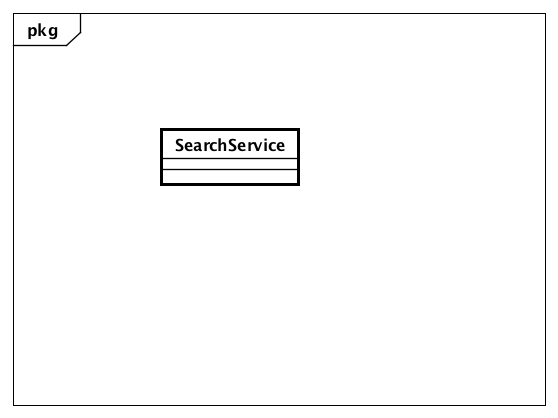
\includegraphics[scale=0.45]{UML/Classi/Front-End/QuizziPedia_Front-end_Services_ SearchService.png}
	\caption{QuizziPedia::Front-End::Services::LangService}
\end{figure}
\begin{itemize}
	\item \textbf{Descrizione}: questa classe permette di gestire il recupero dei dati dal back-end a seguito di una ricerca effettuata da un utente;
	\item \textbf{Utilizzo}: fornisce le funzionalità per recuperare dal back-end delle informazioni basandosi sulle keyword inserite dall'utente;
	\item \textbf{Relazione con altre classi:}
	\begin{itemize}
		\item \textit{OUT} \texttt{SearchController}: ;
	\end{itemize}
	\item \textbf{Attributi:}
	\begin{itemize}
		\item \texttt{-} \texttt{\$http: \$http}: campo dati che contiene un riferimento al servizio \$http che permette la comunicazione con il protocollo HTTP;
		\item \texttt{-} \texttt{\$q: \$q}: campo dati che contiene un riferimento a \$q, un servizio offerto da \textit{Angular\ped{G}} per la gestione, tramite \textit{Promise\ped{G}}, di chiamate asincrone. 
	\end{itemize}
	\item \textbf{Metodi:}
	\begin{itemize}
		\item \texttt{+} \texttt{Search(keyword: String): Promise} \\Metodo che serve per recuperare la lista di utenti e questionari dopo una ricerca. Il metodo ritorna una \textit{Promise\ped{G}}. In caso la \textit{Promise\ped{G}} venga rifiutata, verrà restituito al \texttt{SearchController} un oggetto \texttt{ErrorModelInfo} contenente tutti i dettagli dell'errore. \\
		\textbf{parametri}:
		\begin{itemize}
			\item \texttt{keyword: String}: parametro rappresenta la parola da cercare.
		\end{itemize}
	\end{itemize}
\end{itemize}

\paragraph{QuizziPedia::Front-End::Services::LangService}
\begin{figure}
	\centering
	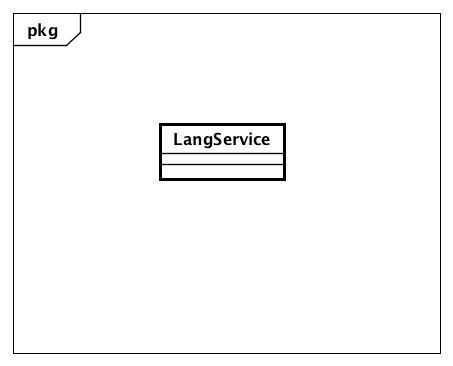
\includegraphics[scale=0.45]{UML/Classi/Front-End/QuizziPedia_Front-end_Services_ LangService.png}
	\caption{QuizziPedia::Front-End::Services::LangService}
\end{figure}
\begin{itemize}
	\item \textbf{Descrizione}: questa classe permette di gestire la lingua nella quale si è scelto di utilizzare l'applicazione.
	\item \textbf{Utilizzo}: fornisce delle funzionalità per recuperare la giusta traduzione della pagina.
	\item \textbf{Relazione con altre classi:}
	\begin{itemize}
		\item \textit{IN} \texttt{AppRun}
	\end{itemize}
	\item \textbf{Attributi:}
	\begin{itemize}
		\item \texttt{-} \texttt{\$http: \$http}: campo dati che contiene un riferimento al servizio \$http che permette la comunicazione con il protocollo HTTP;
	\end{itemize}
	\item \textbf{Metodi:}
	\begin{itemize}
		\item \texttt{+} \texttt{getKeywords(): Object}: \\Metodo che ritorna la lista di tutte le keywords nella lingua richiesta.\\
		\textbf{Parametri}:
		\begin{itemize}
			\item \texttt{lang: String}: parametro che indica la lingua delle keywords da restituire.
		\end{itemize}
	\end{itemize}
\end{itemize}

\paragraph{QuizziPedia::Front-End::Services::QuizService}
\begin{figure}
	\centering
	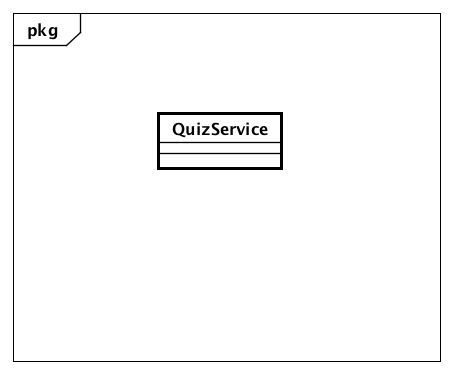
\includegraphics[scale=0.45]{UML/Classi/Front-End/QuizziPedia_Front-end_Services_ QuizService.png}
	\caption{QuizziPedia::Front-End::Services::QuizService}
\end{figure}
\begin{itemize}
	\item \textbf{Descrizione}: questa classe permette di ottenere i dati di un quiz tramite delle parole chiave inserite dall'utente nella barra di ricerca. Permette inoltre di iscriversi ad un questionario e di scaricare l'intera l'ista di domande di un questionario a partire dal suo id univoco;
	\item \textbf{Utilizzo}: fornisce le funzionalità per ottenere i dati di un quiz in seguito ad una ricerca dell'utente, passando i risultati ai controllers. Ritorna dei riferimenti alle domande del quiz;
	\item \textbf{Relazione con altre classi:}
	\begin{itemize}
		\item \textit{OUT} \texttt{SearchController}: questa classe permette di gestire la ricerca di questionari e utenti all'interno dell'applicazione;
		\item \textit{OUT} \texttt{QuestionsController}: questa classe permette di gestire il recupero delle domande per poterle stampare nella modalità allenamento;
		\item \textit{OUT} \texttt{QuestionnaireDetailsController}: questa classe permette di gestire i dettagli di un questionario;
		\item \textit{OUT} \texttt{FillingQuestionnaireController}: questa classe permette di gestire la compilazione del questionario;
		\item \textit{OUT} \texttt{CreateQuestionnaireController}: questa classe permette di gestire la creazione di un questionario;
		\item \textit{OUT} \texttt{RegistrationManagementController}: questa classe permette di gestire le iscrizione degli utenti ai questionari;
		\item \textit{OUT} \texttt{ResultsController}: questa classe permette di gestire le iscrizione degli utenti ai questionari; 
		\item \textit{OUT} \texttt{QuestionnaireManagementController}: questa classe permette di gestire tutti i questionari creati da un utente. 
		
	\end{itemize}
	\item \textbf{Attributi:}
	\begin{itemize}
		\item \texttt{-} \texttt{\$http: \$http}: campo dati che contiene un riferimento al servizio \$http che permette la comunicazione con il protocollo HTTP;
		\item \texttt{-} \texttt{\$q: \$q}: campo dati che contiene un riferimento a \$q, un servizio offerto da \textit{Angular\ped{G}} per la gestione, tramite \textit{Promise\ped{G}}, di chiamate asincrone.
	\end{itemize}
	\item \textbf{Metodi:} \\
	\item \texttt{+} \texttt{Search(quizId: String): Promise} \\Metodo che serve per recuperare i questionari dopo averne selezionato uno dalla lista ottenuta da una ricerca. Il metodo ritorna una \textit{Promise\ped{G}}. In caso la \textit{Promise\ped{G}} venga rifiutata, verrà restituito al \texttt{SearchController} un oggetto \texttt{ErrorModelInfo} contenente tutti i dettagli dell'errore. \\
	\textbf{parametri}:
	\begin{itemize}
		\item \texttt{quizId: String}: parametro che rappresenta il questionario da cercare.
	\end{itemize}
	\item \texttt{+} \texttt{subscribeQuestionnaire(username: String)}: \\Metodo per iscriversi ad un questionario;
	\begin{itemize}
		\item \texttt{username: String}: parametro che rappresenta l'utente da registrare al questionario;
	\end{itemize}
	\item \texttt{+} \texttt{getQuestionnaireDetails(username: String): Promise}: \\Metodo che serve per ritornare i dettagli di tutti i questionari creati da un utente; Il metodo ritorna una \textit{Promise\ped{G}}. In caso la \textit{Promise\ped{G}} venga rifiutata, verrà restituito al \texttt{StatisticsController} un oggetto \texttt{ErrorModelInfo} contenente tutti i dettagli dell'errore. \\ 
	\begin{itemize}
		\item \texttt{username: String}: parametro che rappresenta l'utente del quale andranno caricati tutti i questionari;
	\end{itemize}
	\item \texttt{getDoneQuestionnaire(username: String): Promise}: \\ Metodo che restituisce tutti i questionari svolti da un utente. Il metodo ritorna una \textit{Promise\ped{G}}. In caso la \textit{Promise\ped{G}} venga rifiutata, verrà restituito al \texttt{UserDetailsController} un oggetto \texttt{ErrorModelInfo} contenente tutti i dettagli dell'errore. \\ 
	\begin{itemize}
		\item \texttt{username: String}: parametro che rappresenta l'utente del quale andranno caricati tutti i questionari svolti;
	\end{itemize}
	\item \texttt{createQuestionnaire(title: String, questions: QuestionnaireItemModel): Promise}: \\ Metodo che permette di creare un nuovo questionario. Il metodo ritorna una \textit{Promise\ped{G}}. In caso la \textit{Promise\ped{G}} venga rifiutata, verrà restituito al \texttt{CreateQuestionnaireController} un oggetto \texttt{ErrorModelInfo} contenente tutti i dettagli dell'errore. \\
	\textbf{parametri}:
	\begin{itemize}
		\item \texttt{title: String}: parametro che rappresenta il titolo del questionario.
		\item \texttt{questions: QuestionnaireItemModel}: parametro contenente tutte le domande del questionario;
	\end{itemize}
\end{itemize}

\paragraph{QuizziPedia::Front-End::Services::StatisticsService}
\begin{figure}
	\centering
	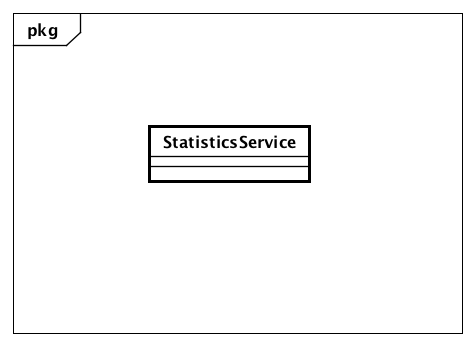
\includegraphics[scale=0.45]{UML/Classi/Front-End/QuizziPedia_Front-end_Services_ StatisticsService.png}
	\caption{QuizziPedia::Front-End::Services::StatisticsService}
\end{figure}
\begin{itemize}
	\item \textbf{Descrizione}: questa classe permette di ottenere le statistiche dell'utente;
	\item \textbf{Utilizzo}: fornisce al controller le statistiche salvate;
	\item \textbf{Relazione con altre classi:}
	\begin{itemize}
		\item \textit{IN} \texttt{StatisticsController}: questa classe permette di le statistiche di un utente.
	\end{itemize}
	\item \textbf{Attributi:}
	\begin{itemize}
		\item \texttt{-} \texttt{\$http: \$http}: campo dati che contiene un riferimento al servizio \$http che permette la comunicazione con il protocollo HTTP;
		\item \texttt{-} \texttt{\$q: \$q}: campo dati che contiene un riferimento a \$q, un servizio offerto da \textit{Angular\ped{G}} per la gestione, tramite \textit{Promise\ped{G}}, di chiamate asincrone.
	\end{itemize}
	\item \textbf{Metodi:}
	\begin{itemize}
		\item \texttt{+} \texttt{getStatistics(username: String): Promise}: \\Metodo che serve per recuperare le statistiche di un utente tramite chiamata al back-end. Il metodo ritorna una \textit{Promise\ped{G}}. In caso la \textit{Promise\ped{G}} venga rifiutata, verrà restituito al \texttt{StatisticsController} un oggetto \texttt{ErrorModelInfo} contenente tutti i dettagli dell'errore. \\
		\begin{itemize}
			\item \texttt{username: String}: parametro che indica l'utente del quale andranno caricate tutte le statistiche;
		\end{itemize}
		\item \texttt{+} \texttt{getQuestionnaireStatistics(quizId: String): Promise} \\Metodo che restituisce le statistiche di un questionario.  Il metodo ritorna una \textit{Promise\ped{G}}. In caso la \textit{Promise\ped{G}} venga rifiutata, verrà restituito al \texttt{StatisticsController} un oggetto \texttt{ErrorModelInfo} contenente tutti i dettagli dell'errore. \\
		\begin{itemize}
			\item \texttt{quizId: String}: parametro che indica il questionario del quale verranno caricate le statistiche;
		\end{itemize}
	\end{itemize}
\end{itemize}

\paragraph{QuizziPedia::Front-End::Services::QuestionsServices}
\begin{figure}
	\centering
	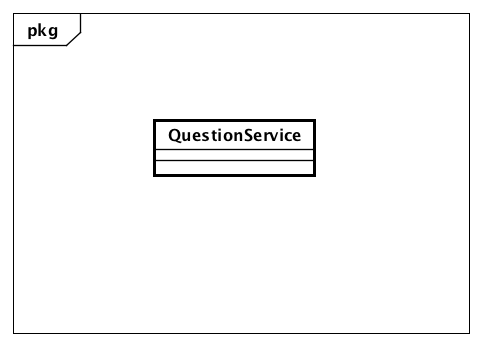
\includegraphics[scale=0.45]{UML/Classi/Front-End/QuizziPedia_Front-end_Services_ QuestionService.png}
	\caption{QuizziPedia::Front-End::Services::QuestionService}
\end{figure}
\begin{itemize}
	\item \textbf{Descrizione}: questa classe permette di ottenere domande esistenti e salvare nuove domande;
	\item \textbf{Utilizzo}: utilizzata per richiedere domande presenti nel database. Offre inoltre delle funzionalità per inserire nuove domande;
	\item \textbf{Relazione con altre classi:}
	\begin{itemize}
		\item \textit{IN} \texttt{TrueFalseQuestionsController}: questa classe permette di gestire la creazione e la modifica di una domanda vero/falso;
		\item \textit{IN} \texttt{MultiplyQuestionsController}: questa classe permette di gestire la creazione e la modifica di una domanda a risposta multipla; 
		\item \textit{IN} \texttt{ConnectionQuestionsController}: questa classe permette di gestire la creazione e la modifica di una domanda a collegamento;
		\item \textit{IN} \texttt{ImagesSortingQuestionsController}: questa classe permette di gestire la creazione e la modifica di una domanda a ordinamento immagini;
		\item \textit{IN} \texttt{StringsSortingQuestionsController}: questa classe permette di gestire la creazione e la modifica di una domanda a ordinamento di stringhe;
		\item \textit{IN} \texttt{FillingQuestionsController}: questa classe permette di gestire la creazione e la modifica di una domanda a riempimento di spazi; 
		\item \textit{IN} \texttt{ClickableAreaQuestionsController}: questa classe permette di gestire la creazione e la modifica di una domanda ad area cliccabile;
		\item \textit{IN} \texttt{EditorQMLController}: questa classe permette di gestire la creazione e la modifica di domande create tramite editor QML;
		\item \textit{IN} \texttt{QuestionsManagementController}: questa classe permette di gestire e di ottenere le domande create dall'utente
		\item \textit{IN} \texttt{TopicKeywordsController}: questa classe permette di gestire il recupero delle parole chiave di un questionario;
		\item \textit{IN} \texttt{QuestionnaireQuestionsManagementController}: questa classe permette di gestire il recupero delle domande per il questionario;
		\item \textit{IN} \texttt{QuestionsController}: questa classe permette di gestire il recupero delle domande per poterle stampare nella modalità allenamento.
		
	\end{itemize}
	\item \textbf{Attributi:}
	\begin{itemize}
		\item \texttt{-} \texttt{\$http: \$http}: campo dati che contiene un riferimento al servizio \$http che permette la comunicazione con il protocollo HTTP;
		\item \texttt{-} \texttt{\$q: \$q}: campo dati che contiene un riferimento a \$q, un servizio offerto da \textit{Angular\ped{G}} per la gestione, tramite \textit{Promise\ped{G}}, di chiamate asincrone.
	\end{itemize}
	\item \textbf{Metodi:}
	\begin{itemize}
		\item \texttt{+} \texttt{sendQuestion(type: String, lang: String, text: String, image: ?, answer: String[]): Promise}: \\Metodo che serve per mandare una domanda al back-end in modo che venga salvata;\\ 
		\textbf{Parametri}: 
		\begin{itemize}
			\item \texttt{type: String}: identifica la tipologia della domanda;
			\item \texttt{lang: String}: identifica la lingua della domanda;
			\item \texttt{text: String}: identifica il testo della domanda;
			\item \texttt{image: ?}: identifica un'immagine associata alla domanda;
			\item \texttt{answer: String[]}: identifica l'array delle risposte alla domanda.
		\end{itemize}
		\item \texttt{+} \texttt{getUserQuestions(username: String): Promise}: \\Metodo che ritorna tutte le domande create dall'utente. Il metodo ritorna una \textit{Promise\ped{G}}. In caso la \textit{Promise\ped{G}} venga rifiutata, verrà restituito al \texttt{QuestionsController} un oggetto \texttt{ErrorModelInfo} contenente tutti i dettagli dell'errore. \\
		\begin{itemize}
			\item \texttt{username: String}: parametro che indica l'utente del quale andranno caricate tutte le domande da lui create;
		\end{itemize}
	\end{itemize}
\end{itemize}

\paragraph{QuizziPedia::Front-End::Services::UserDetailsService}
\begin{figure}
	\centering
	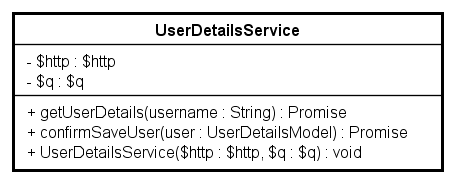
\includegraphics[scale=0.45]{UML/Classi/Front-End/QuizziPedia_Front-end_Services_UserDetailsService.png}
	\caption{QuizziPedia::Front-End::Services::UserDetailsService}
\end{figure}
\begin{itemize}
	\item \textbf{Descrizione}: questa classe permette di ottenere i dati personali degli utenti;
	\item \textbf{Utilizzo}: utilizzata per ottenere i dati personali di un utente. Permette inoltre di trovare i dati di utenti ricercati tramite l'apposita barra di ricerca;
	\item \textbf{Relazione con altre classi:}
	\begin{itemize}
		\item \textit{OUT} \texttt{SearchController}: questa classe permette di gestire la ricerca di questionari e utenti all'interno dell'applicazione;
		\item \textit{OUT} \texttt{UserDetailsController}: questa classe permette di gestire i dati di un utente;
		\item \textit{OUT} \texttt{ProfileManagementController}: questa classe permette di gestire il profilo personale di un utente. 
	\end{itemize}
	\item \textbf{Attributi:}
	\begin{itemize}
		\item \texttt{-} \texttt{\$http: \$http}: campo dati che contiene un riferimento al servizio \$http che permette la comunicazione con il protocollo HTTP;
		\item \texttt{-} \texttt{\$q: \$q}: campo dati che contiene un riferimento a \$q, un servizio offerto da \textit{Angular\ped{G}} per la gestione, tramite \textit{Promise\ped{G}}, di chiamate asincrone.
	\end{itemize}
	\item \textbf{Metodi:}
	\begin{itemize}
		\item \texttt{+} \texttt{getUserDetails(username: String): Promise} \\ Metodo che serve per ottenere i dettagli di un utente. Il metodo ritorna una \textit{Promise\ped{G}}. In caso la \textit{Promise\ped{G}} venga rifiutata, verrà restituito al \texttt{SearchController} un oggetto \texttt{ErrorModelInfo} contenente tutti i dettagli dell'errore. \\
		\begin{itemize}
			\item \texttt{username: String}: parametro che indica l'utente del quale andranno caricati tutti i dati personali;
		\end{itemize}
		\item \texttt{+} \texttt{confirmSaveUser(user: UserDetailsModel): Promise} \\Metodo che serve per inviare al back-end una richiesta di salvataggio persistente dei dati. Viene invocato da Confirm in SearchController. Il metodo ritorna una \textit{Promise\ped{G}}. In caso la \textit{Promise\ped{G}} venga rifiutata, verrà restituito al \texttt{SearchController} un oggetto \texttt{ErrorModelInfo} contenente tutti i dettagli dell'errore. \\
		\begin{itemize}
			\item \texttt{user: UserDetailModel}: parametro che indica l'oggetto contenente tutti i dati dell'utente che dovranno essere salvati dal back-end;
		\end{itemize}
	
	\end{itemize}
\end{itemize}
